\documentclass[10pt]{amsart}
\usepackage[a4paper,margin=22mm]{geometry}
\usepackage[no-math]{fontspec}
\setmainfont{Latin Modern Roman}[SmallCapsFont={lmromancaps10-regular.otf}]
\usepackage{amsmath,amssymb,amsthm,mathtools,hyperref,graphicx,float,etoolbox}
\usepackage[shortlabels]{enumitem}
\emergencystretch=3em
\newtheorem{theo}{Theorem}[section]
\newtheorem{lemm}[theo]{Lemma}
\newtheorem{prop}[theo]{Proposition}
\newtheorem{coro}[theo]{Corollary}
\theoremstyle{definition}
\newtheorem{defi}[theo]{Definition}
\newtheorem{rema}[theo]{Remark}
\newtheorem{exam}[theo]{Example}
\numberwithin{figure}{section}
\usepackage{tcolorbox}
\usepackage{bbm}
\usepackage{tikz}





%\providecommand{\R}{}
%\providecommand{\Z}{}
%\providecommand{\N}{}
%\providecommand{\C}{}
%\providecommand{\Q}{}
%\providecommand{\G}{}
%\providecommand{\Lt}{}
\newcommand{\R}{\mathbb{R}}
\newcommand{\Z}{\mathbb{Z}}
\newcommand{\N}{\mathbb{N}}
\renewcommand{\P}{\mathbb{P}}
\newcommand{\D}{\mathbb{D}}

\newcommand*\W{\mathsf{W}}
\renewcommand{\H}{\mathsf{Height}}
\newcommand{\height}{\mathsf{H}}


\newcommand{\bfs}{\mathsf{bfs}}

\newcommand{\p}{\mathbf{P}}
\newcommand{\bfw}{\mathbf{w}}
\newcommand{\bffs}{\mathbf{s}}
\newcommand{\Width}{\mathsf{Width}}
\newcommand{\lex}{\mathsf{lex}}
\newcommand{\sExp}{\mathsf{Exp}}

\newcommand{\E}[1]{{\mathbf E}\left[#1\right]}
\newcommand{\bfE}{\mathbf{E}}


\newcommand{\sequence}[1]{\mathrm{#1}}
\DeclareMathOperator{\tree}{t}
\DeclareMathOperator{\rtree}{T}
\DeclareMathOperator{\rseq}{V}
\DeclareMathOperator{\dseq}{d}
\DeclareMathOperator{\Dseq}{D}
\DeclareMathOperator{\Sseq}{S}

\DeclareMathOperator{\dxseq}{d\mathit{x}}
\DeclareMathOperator{\duseq}{d\mathit{u}}
\DeclareMathOperator{\dtseq}{d\mathit{t}}

\DeclareMathOperator{\st}{st}
\DeclareMathOperator{\TV}{TV}
\DeclareMathOperator{\rmL}{L}
\DeclareMathOperator{\rmR}{R}
\DeclareMathOperator{\rmH}{H}

\DeclareMathOperator{\gcdd}{gcd}
\newcommand\cA{\mathcal{A}}
\newcommand{\cH}{\mathcal{H}}

\newcommand\cD{\mathcal{D}}
\newcommand{\cF}{\mathcal{F}}
\newcommand{\cC}{\mathcal{C}}
\newcommand{\cV}{\mathcal{V}}
\newcommand\cS{\mathcal{S}}
\newcommand\cT{\mathcal{T}}
\newcommand{\cW}{\mathcal{W}}
\newcommand{\clP}{\mathcal{P}}
\newcommand{\cU}{\mathcal{U}}
\newcommand{\noopsort}[1]{}

%\makeatletter
%\newcommand{\optionaldesc}[2]{
%\phantomsection #1\protected@edef\@currentlabel{#1}\label{#2}
%}
%\makeatother
\newcommand{\I}[1]{{\mathbbm 1}_{#1}}
\newcommand{\set}[1]{\left(#1 \right)}
\newcommand{\Cprob}[2]{\mathbf{P}\set{\left. #1 \; \middle| \; #2\right.}}
\newcommand{\probC}[2]{\mathbf{P}\set{\left. #1 \; \middle| \; #2 \right. }}


\newcommand{\eqdist}{\ensuremath{\stackrel{\mathrm{d}}{=}}}

\providecommand{\eps}{}
\renewcommand{\eps}{\varepsilon}
\providecommand{\ora}[1]{}




\newcommand{\Tn}{\rtree_{n}}

\newcommand{\llbracket}{\mathopen{[\mkern -2.7mu[}}
\newcommand{\rrbracket}{\mathclose{]\mkern -2.7mu]}}

%%%%%%%%%%%%%%%%%%%%%%%%%%%%%%%%%%%%%%%%%%%%%%%%%%%%%%%%%%%%%%%%%%%%%%%%%%%%%%%%%%%%%%%%%%%%%%%%%%%%%%%%%%%%%%
\graphicspath{{./figures/}}

\newcommand*{\mk}{\mkern -1mu}
\newcommand*{\Mk}{\mkern -2mu}
\newcommand*{\mK}{\mkern 1mu}
\newcommand*{\MK}{\mkern 2mu}

\hypersetup{urlcolor=purple, linkcolor=blue, citecolor=red}

\newcommand*{\romanenumi}{\renewcommand*{\theenumi}{\roman{enumi}}}
\newcommand*{\Romanenumi}{\renewcommand*{\theenumi}{\Roman{enumi}}}
\newcommand*{\alphenumi}{\renewcommand*{\theenumi}{\alph{enumi}}}
\newcommand*{\Alphenumi}{\renewcommand*{\theenumi}{\Alph{enumi}}}
\let\oldtilde\tilde
\renewcommand*{\tilde}[1]{\mathchoice{\widetilde{#1}}{\widetilde{#1}}{\oldtilde{#1}}{\oldtilde{#1}}}
\let\oldhat\hat
\renewcommand*{\hat}[1]{\mathchoice{\widehat{#1}}{\widehat{#1}}{\oldhat{#1}}{\oldhat{#1}}}
\title[Critical conditioned trees: height and width]{Critical size-conditioned Bienaym\'e trees have superlogarithmic height and sublinear width without higher moment assumptions}
\author{Louigi Addario-Berry}
\author{Serte Donderwinkel}
\author{Igor Kortchemski}
\date{Annales Henri Lebesgue 8 (2025),113–149; DOI 10.5802/ahl.231}
\hypersetup{hidelinks}
\AtBeginDocument{\let\originalRef\ref\renewcommand{\ref}[1]{\ifstrequal{#1}{fig:bij}{\href{https://doi.org/10.5802/ahl.231}{4.1 (source)}}{\originalRef{#1}}}}
\begin{document}
\maketitle
\section{Introduction}

For a rooted tree $\tree$, the \emph{size} $|\tree|$ of $\tree$ is its number of vertices, the \emph{height} $\H(\tree)$ is the greatest distance of any vertex of $\tree$ from the root, and the \emph{width} $\Width(\tree)$ is the greatest number of nodes in any single generation of $\tree$.

Given a probability measure $\mu$ on $\Z_{+}$ (hereafter referred to as an \emph{offspring distribution}), write $\rtree=\rtree(\mu)$ for a $\mu$-Bienaymé tree, i.e., the family tree of a $\mu$-distributed branching process.\footnote{Also known as \emph{Galton--Watson} or \emph{Bienaymé--Galton--Watson} trees. Here we adopt the nomenclature proposed in~\cite{ABHK21}.} For $n \in \N$ with $\p(|\rtree|=n)>0$, write $\rtree_n=\rtree_n(\mu)$ for a random tree distributed as $\rtree$ conditioned to have size $n$. We prove the following lower bound on $\H(\rtree_n)$, which holds for all offspring distributions $\mu$ that are \emph{critical}, meaning that they have mean~$1$.
\begin{theo}\label{thm:height_critical0}
Let $\mu$ be any critical offspring distribution. Then
\[
\H(\rtree_{n}) = \omega_{\p}(\ln n)
\quad \text{and} \quad
\Width(\rtree_n)=o_{\p}(n).
\]
\end{theo}
The notation $X_n = \omega_{\p}(Y_n)$ means that $X_n/Y_n \to \infty$ in probability as $n \to \infty$; in the theorem (and implicitly in the sequel) the limit is along $n$ for which $\p(|\rtree|=n)>0$.

The proof relies on the powerful Foata--Fuchs bijection, which establishes a connection between trees and sequences. This bijection can be reformulated as a line-breaking construction and we essentially show that for a critical offspring distribution, the longest path used to build the tree has length $\omega_{\p}(\ln n)$.
\section{Bienaymé trees and their coding}\label{sec:trees}

\subsection{Plane trees}\label{sssec:planetrees}

We define plane trees according to Neveu's formalism~\cite{Nev86}. Let $\N = \{1, 2, \dots\}$ be the set of positive integers, and consider the set of labels $\cU = \bigcup_{n\,\ge\,0} \N^n$ (where by convention $\N^0 = \{\varnothing\}$). For every $v = (v_1, \dots, v_n) \in \cU$, the length of $v$ is $\|v\| = n$. For $u,v\in \cU$, we let $uv$ be the concatenation of $u$ and $v$.

Then, a (locally finite) \emph{plane tree} is a nonempty subset $\tree \subset \cU$ satisfying the following conditions. First, $\varnothing \in \tree$ ($\varnothing$ is called the \emph{root vertex} of the tree). Second, if $v=(v_1,\ldots,v_n) \in \tree$ with $n \ge 1$, then $(v_1,\ldots,v_{n-1}) \in \tree$ ($(v_1,\ldots,v_{n-1})$ is called the \emph{parent} of $v$ in $\tree$). Finally, if $v \in \tree$, then there exists an integer $k_v(\tree) \ge 0$ such that $(v_1,\ldots,v_n,i) \in \tree$ if and only if $1 \le i \le k_v(\tree)$. The quantity $k_v(\tree)$ is the \emph{number of children} of $v$ in $\tree$; we also refer to $k_v(\tree)$ as the \emph{degree} of $v$ in $\tree$. The plane tree $\tree$ may be seen as a genealogical tree in which the individuals are the vertices $v\in\tree$.

For $v,w \in \tree$, we let $\llbracket v, w \rrbracket$ be the vertices belonging to the shortest path from $v$ to $w$ in $\tree$. We use $\llbracket v, w \llbracket$ for the set obtained from $\llbracket v, w \rrbracket$ by excluding $w$. We also let $|\tree|$ be the total number of vertices (that is, the size) of the plane tree $\tree$.

\subsection{Coding trees by lattice paths}\label{sssec:coding}
Let $\tree$ be a {finite} plane tree. We associate with every ordering $\varnothing=u_{0}\prec u_{1}\prec \cdots \prec u_{|\tree|-1}$ of the vertices of $\tree$ the path $\W(\tree)=(\W_n(\tree) : 0 \leq n < |\tree|)$, defined by $ \W_0(\tree)=0$, and $ \W_{n+1}(\tree)= \W_{n}(\tree)+k_{u_n}(\tree)-1$ for every $0 \leq n < |\tree|$.

We will use two different orderings of the vertices of a tree:
\begin{enumerate}\romanenumi
\item the lexicographical ordering, where $v \prec w$ if there exists $u \in \cU$ such that $v = u(v_1, \dots, v_n)$, $w = u(w_1, \dots, w_m)$ and $v_1 < w_1$;
\item the breadth-first search ordering, where $v \prec w$ if either $\|v\| <\|w\|$, or $\|v\|=\|w\|$ and $v=u(v_1, \dots, v_m)$ and $w=u (w_1, \dots, w_m)$ with $v_{1}<w_{1}$.
\end{enumerate}

Denote by $\W^{\lex}(\tree)$ and $\W^{\bfs}(\tree)$ the paths constructed by using respectively the lexicographical and breadth-first search ordering of the vertices of $ \tree$. We refer to both $\W^{\lex}$ and $\W^{\bfs}$ as \emph{exploration processes}; we call $\W^{\lex}(\tree)$ the \emph{{\L}ukasiewicz path} of $ \tree$ and $\W^{\bfs}(\tree)$ the \emph{breadth-first queue process} of~$\tree$.

The following deterministic fact will be useful. Let $\tree$ be a finite tree and order the vertices of $\tree$ using the breadth-first search ordering as $u_0,\dots,u_{|\tree|-1}$. Then for every $1 \le i \le |\tree|$, writing $\ell=\|u_{i-1}\|$, then $\W^{\bfs}_{{i}}(\tree)$ is equal to the total number of children of generation-$\ell$ predecessors of $u_{i-1}$ plus the number of generation-$\ell$ successors of $u_{i-1}$ (where ``predecessor'' and ``successor'' are relative to the breadth-first search order).


As a consequence,
\begin{equation}\label{eq:width}
\Delta(\tree) \leq \Width(\tree) \leq \max\left(\W^{\bfs}_i(\tree), 0 \le i < |t|\right),
\end{equation}
where we define $\Delta(\tree)=\max_{u\,\in\,\tree} k_{u}(\tree)$ to be the maximal number of children of a vertex.



Set $[n]=\{1,2,\dots, n\}$. A \emph{discrete bridge of length $n$} is a lattice path $\bffs=(s_0,\ldots,s_n)$ with $s_0=0$ and $s_n=-1$ and $s_{i}-s_{i-1} \ge -1$ for $i \in [n]$; it is a \emph{discrete excursion} if additionally $s_i \ge 0$ for $i \in [n-1]$.

For either $\ast \in \{\lex,\bfs\}$ and any $n \ge 1$, the map
\[
\tree \mapsto \W^{\ast}(\tree)
\]
induces an invertible function with domain the set of plane trees with $n$ vertices and range the set of discrete excursions of length $n$.

The \emph{Vervaat transform} is an $n$-to-$1$ map from discrete bridges of length $n$ to discrete excursions of length n which is defined as follows. Let $\bffs=(s_i : 0 \leq i \leq n)$ be a discrete bridge, and for $1 \le i \le n$ let $x_i=s_i-s_{i-1}$. Also, let
\[
m=m(\bffs)\coloneqq\min\big\{0\leq i \leq n : s_i=\min\{s_j : 0\leq j \leq n\}\big\}.
\]
be the first time at which $(s_i : 0\leq i \leq n)$ reaches its overall minimum. Then the Vervaat transform $\cV(\bffs) \coloneqq (\cV(\bffs)_i : 0\leq i \leq n)$ of $\bffs$ is the walk obtained by reading the increments $(x_1,\ldots, x_n)$ from left to right in cyclic order, started from $m$. Namely,
\[
\cV(\bffs)_0=0 \quad \text{and} \quad \cV(\bffs)_{i+1}-\cV(\bffs)_{i}= x_{m+i \mod[n]}, \quad 0\leq i < n.
\]
See Figure~\ref{fig:vervaat} for an illustration.

\begin{figure}[h!]
\begin{center}
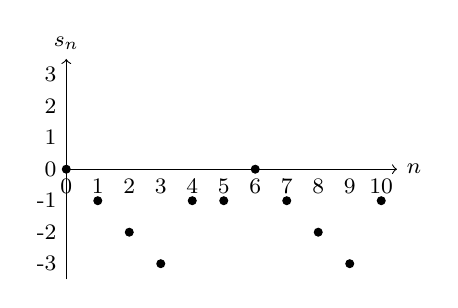
\begin{tikzpicture}[scale = 0.4]
\draw[->] (0,-3.5) -- (0,3.5);
\draw[->] (0,0) -- (10.5,0);

\node[above,font=\footnotesize] at (0,3.5) {$s_n$};
\node[right,font=\footnotesize] at (10.5,0) {$n$};

\node[draw,circle,fill,inner sep = 1pt] at (0,0) {};
\node[draw,circle,fill,inner sep = 1pt] at (1,-1) {};
\node[draw,circle,fill,inner sep = 1pt] at (2,-2) {};
\node[draw,circle,fill,inner sep = 1pt] at (3,-3) {};
\node[draw,circle,fill,inner sep = 1pt] at (4,-1) {};
\node[draw,circle,fill,inner sep = 1pt] at (5,-1) {};
\node[draw,circle,fill,inner sep = 1pt] at (6,0) {};
\node[draw,circle,fill,inner sep = 1pt] at (7,-1) {};
\node[draw,circle,fill,inner sep = 1pt] at (8,-2) {};
\node[draw,circle,fill,inner sep = 1pt] at (9,-3) {};
\node[draw,circle,fill,inner sep = 1pt] at (10,-1) {};


\node[left,font=\footnotesize] at (0,-1) {-1};
\node[left,font=\footnotesize] at (0,-2) {-2};
\node[left,font=\footnotesize] at (0,-3) {-3};
\node[left,font=\footnotesize] at (0,0) {0};
\node[left,font=\footnotesize] at (0,1) {1};
\node[left,font=\footnotesize] at (0,2) {2};
\node[left,font=\footnotesize] at (0,3) {3};

\node[below,font=\footnotesize] at (0,0) {0};
\node[below,font=\footnotesize] at (1,0) {1};
\node[below,font=\footnotesize] at (2,0) {2};
\node[below,font=\footnotesize] at (3,0) {3};
\node[below,font=\footnotesize] at (4,0) {4};
\node[below,font=\footnotesize] at (5,0) {5};
\node[below,font=\footnotesize] at (6,0) {6};
\node[below,font=\footnotesize] at (7,0) {7};
\node[below,font=\footnotesize] at (8,0) {8};
\node[below,font=\footnotesize] at (9,0) {9};
\node[below,font=\footnotesize] at (10,0) {10};
\end{tikzpicture}
\quad
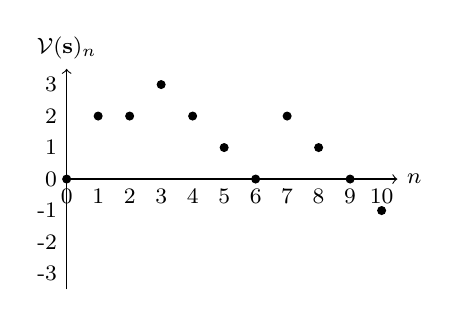
\begin{tikzpicture}[scale = 0.4]
\draw[->] (0,-3.5) -- (0,3.5);
\draw[->] (0,0) -- (10.5,0);

\node[above,font=\footnotesize] at (0,3.5) {$\cV(\bffs)_n$};
\node[right,font=\footnotesize] at (10.5,0) {$n$};

\node[draw,circle,fill,inner sep = 1pt] at (0,0) {};
\node[draw,circle,fill,inner sep = 1pt] at (1,2) {};
\node[draw,circle,fill,inner sep = 1pt] at (2,2) {};
\node[draw,circle,fill,inner sep = 1pt] at (3,3) {};
\node[draw,circle,fill,inner sep = 1pt] at (4,2) {};
\node[draw,circle,fill,inner sep = 1pt] at (5,1) {};
\node[draw,circle,fill,inner sep = 1pt] at (6,0) {};
\node[draw,circle,fill,inner sep = 1pt] at (7,2) {};
\node[draw,circle,fill,inner sep = 1pt] at (8,1) {};
\node[draw,circle,fill,inner sep = 1pt] at (9,0) {};
\node[draw,circle,fill,inner sep = 1pt] at (10,-1) {};


\node[left,font=\footnotesize] at (0,-1) {-1};
\node[left,font=\footnotesize] at (0,-2) {-2};
\node[left,font=\footnotesize] at (0,-3) {-3};
\node[left,font=\footnotesize] at (0,0) {0};
\node[left,font=\footnotesize] at (0,1) {1};
\node[left,font=\footnotesize] at (0,2) {2};
\node[left,font=\footnotesize] at (0,3) {3};

\node[below,font=\footnotesize] at (0,0) {0};
\node[below,font=\footnotesize] at (1,0) {1};
\node[below,font=\footnotesize] at (2,0) {2};
\node[below,font=\footnotesize] at (3,0) {3};
\node[below,font=\footnotesize] at (4,0) {4};
\node[below,font=\footnotesize] at (5,0) {5};
\node[below,font=\footnotesize] at (6,0) {6};
\node[below,font=\footnotesize] at (7,0) {7};
\node[below,font=\footnotesize] at (8,0) {8};
\node[below,font=\footnotesize] at (9,0) {9};
\node[below,font=\footnotesize] at (10,0) {10};
\end{tikzpicture}
\quad
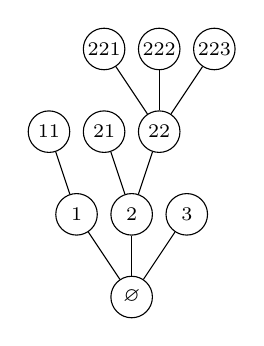
\begin{tikzpicture}[scale = 0.7,
sommet/.style = {draw,circle, font=\scriptsize,inner sep=0,minimum size=15pt}, etiquete/.style = {font = \scriptsize}]

\node[sommet] (0) at (0,0) {$\varnothing$};
\node[sommet] (1) at (-1,1.5) {$1$};
\node[sommet] (2) at (0,1.5) {$2$};
\node[sommet] (3) at (1,1.5) {$3$};
\node[sommet] (11) at (-1.5,3) {$11$};
\node[sommet] (21) at (-0.5,3) {$21$};
\node[sommet] (22) at (0.5,3) {$22$};
\node[sommet] (221) at (-0.5,4.5) {$221$};
\node[sommet] (222) at (0.5,4.5) {$222$};
\node[sommet] (223) at (1.5,4.5) {$223$};

\draw (0) -- (1);
\draw (0) -- (2);
\draw (0) -- (3);
\draw (1) -- (11);
\draw (2) -- (21);
\draw (2) -- (22);
\draw (22) -- (221);
\draw (22) -- (222);
\draw (22) -- (223);
\end{tikzpicture}
\end{center}
\caption{Left: A walk $\bffs=(s_0,\ldots,s_{10})$ with $s_{10}=-1$. Centre: the Vervaat transform $\cV(\bffs)$. Right: the plane tree $\tree$ with $\W^{\bfs}(\tree)=\cV(\bffs)$.}\label{fig:vervaat}
\end{figure}


Let $\mu$ be a critical or subcritical offspring distribution. The Bienaymé measure with offspring distribution $\mu$ is the probability measure $\P_\mu$ on plane trees that is characterized by
\begin{equation}\label{eq:def_GW}
\P_\mu(\tree) = \prod_{u\,\in\,\tree} \mu_{k_u(\tree)}
\end{equation}
for every finite plane tree $\tree$ (see~\cite[Proposition~1.4]{LG05}); in particular, $\rtree(\mu)$ has law~$\P_\mu$.

The following result relates the exploration processes of $\rtree(\mu)$ to a random walk (see~\cite[Proposition~1.5]{LG05} and/or~\cite[Chapter~5 Exercise~1]{MR2245368}). From this point on, $(X_{i} : i \geq 1)$ will always denote a sequence of i.i.d. random variables with law given by $\P(X_{1}=i)=\mu_{i+1}$ for $i \geq -1$ for some offspring distribution $\mu$, and we will always write $S_0=0$ and $S_i=X_1+\ldots+X_i$ for $i \ge 1$. Also, let $\zeta=\inf\{i \ge 1: S_i = -1\}$.
\begin{prop}\label{prop:GWRW}
Fix a critical or subcritical offspring distribution $\mu$ with $\mu_0>0$. Then with $\rtree=\rtree(\mu)$, for every $\ast \in \{\lex,\bfs\}$ we have
\[
\left(\W^{\ast}_{i}(\rtree),0 \le i \le |\rtree|\right)\eqdist (S_i,0 \le i \le \zeta)\,.
\]
Moreover, for any $n \in \N$ the following holds. For any discrete excursion $\bfw=(w_0,\ldots,w_n)$,
\[
\Cprob{(S_i,0 \le i \le n)=\bfw}{\zeta=n} =\Cprob{\cV(S_i,0 \le i \le n)=\bfw}{S_n=-1}\,.
\]
\end{prop}

Together the two identities of Proposition~\ref{prop:GWRW} imply that for $\rtree_n=\rtree_n(\mu)$, we have
\begin{equation}\label{eq:condition_identity}
\p\left((\W^{\ast}_{i}(\rtree_n),0 \le i \le n)=\bffs\right) =
\Cprob{\cV(S_i,0 \le i \le n)=\bfw}{S_n=-1}.
\end{equation}

The following fact follows readily from~\eqref{eq:condition_identity}.
\begin{rema}\label{rk:degrees}
The multiset of degrees in $\rtree_n$ has the same law as the conditional law of the multiset $\{X_i+1,1 \le i \le n\}$ given that $S_n=-1$.
\end{rema}



\setcounter{section}{3}
\section{The height {and width} of large conditioned critical Bienaymé trees}\label{sec:height_critical}
In this section we will prove Theorem~\ref{thm:height_critical0}.


\subsection{Degree sequences of Bienaymé trees}\label{ssec:deg_seq_bien}
We first establish some properties concerning degree sequences of Bienaymé trees {that will be instrumental in our proof of Theorem~\ref{thm:height_critical0}.}


We shall use the following fact about unconditioned samples from $\mu$, which can be found in~\cite[Lemmas~14.3 and~14.4]{Jan12}. We provide a proof for completeness and since our argument is {more probabilistic in nature and also} somewhat shorter than that in~\cite{Jan12}.
\begin{lemm}\label{lem:probtree}
For $(X_i,i \ge 1)$ i.i.d. samples with law $\P(X_1=i)=\mu_{i+1}$, we have that
\[
\P\left(\sum_{i=1}^n X_i=-1\right)=e^{-o(n)}
\]
as $n\to \infty$ over all $n$ for which $\P\left(\sum_{i=1}^n X_i=-1\right)>0$.
\end{lemm} This lemma implies that every event that is exponentially unlikely for $\rtree$ is also exponentially likely for $\rtree_n$. Indeed, by the ballot theorem (or equivalently by Proposition~\ref{prop:GWRW} and the fact that the Vervaat transform is an $n$-to-$1$ map),
\[
\P_\mu(|\rtree|=n)=\frac{1}{n}\P\left(\sum_{i=1}^n X_i=-1\right),
\]
which implies that for any set $\cA$ of plane trees,
\[
\P_\mu(\rtree_{n} \in \cA)\leq \frac{\P(\rtree \in \cA)}{\P_\mu(|\rtree|=n)}\leq ne^{o(n)} \P(\rtree \in \cA).
\]

\begin{proof}[Proof of Lemma~\ref{lem:probtree}]
In the proof, we only consider $n$ for which $\P(\sum_{i=1}^n X_i=-1)>0$.

Now, let $r=\gcdd(i> 0 :\mu_{i}>0)$, so that the support of $\sum_{i=1}^n X_i$ is contained in $-n+r\Z$. Then, there is $k\in \N$ such that $r=\gcdd(0\leq i\leq k:\mu_i>0)$. Set $\cS=\{0\leq i\leq k:\mu_i>0\}$ and let $\cS'=\{i>k :\mu_i>0\}$. If $\cS'=\emptyset$, then we are done, because this in particular implies that $\mu$ has finite variance, so by the local central limit theorem (see e.g.~\cite[Theorem~1, Section~VII]{Petrov}),
\[
\P\left(\sum_{i=1}^n X_i=-1\right)=\Theta(n^{-1/2})
\]
as $n\to \infty$ over all $n$ for which $\P\left(\sum_{i=1}^n X_i=-1\right)>0$. Therefore, we may assume that $\cS'\neq \emptyset$.

Set $p=\sum_{i\,\in\,\cS} \mu_{i}$. Then for $N_{n}\coloneqq\#\{1\leq i \leq n: X_i+1\in \cS\}$, we see that $N_{n}$ is distributed as a $\operatorname{Binomial}(n,p)$ random variable. Moreover, letting $(A_i,i \ge 1)$ be i.i.d. random variables distributed as $X_1$ conditional on $X_1+1\in \cS$ and $(A'_i,i \ge 1)$ be i.i.d. random variables distributed as $X_1$ conditional on $X_1+1 \in \cS'$, both sequences independent of one another and of $N_n$, then
\[
\sum_{i=1}^{N_{n}}A_i+\sum_{i=1}^{n-N_{n}}A'_i  \overset{d}{=}  \sum_{i=1}^n X_i
\]
Let $c=\E{A_1}<0$ and $c'=\E{A'_1}>0$ be the means of $A_1$ and $A'_1$ respectively, which satisfy that $pc+(1-p)c'=0$ by the criticality condition.


Fix $\varepsilon>0$. We are done if we show that
\[
\P\left(\sum_{i=1}^n X_i=-1\right)\geq \tfrac{1}{4} e^{-\varepsilon n}
\]
for all $n$ large enough. To this end, we first observe that there is $M>0$ such that $\P(|N_{n}-np|<Mn^{1/2})>1/2$ for all $n$. Furthermore, since $\sum_{i=1}^mA_i$ is the sum of i.i.d\ random variables with mean $c$ and finite support, there exists $\delta>0$ such that for all $m_n$ with $|m_n-np|<Mn^{1/2}$ and for all $k_n\in -m_n+ r\Z$ with $|k_n-npc|<\delta n$, for all $n$ large enough,
\begin{equation}\label{eq:A}
\P\left(\sum_{i=1}^{m_n}A_i=k_n\right)\geq e^{-\varepsilon n}.
\end{equation}

We now check that for $n$ large enough and for all $m_n$ with $|m_n-np|<Mn^{1/2}$
\begin{equation}\label{eq:Aprime}
\P \left(\left|\sum_{i=1}^{n-m_n}A'_i +npc +1 \right| \leq \delta n \right) \geq \frac{1}{2}.
\end{equation}
Then, with probability at least $\tfrac14$, we get that $m_n=N_n$ and $k_n=-1-\sum_{i=1}^{n-m_n}A'_i$ satisfy the conditions of~\eqref{eq:A}. (Observe that since $\P(\sum_{i=1}^n X_i=-1)>0$ we have that $n-1\in r\Z$, and $\sum_{i=1}^{n-m_n}A'_i\in -n+m_n+r\Z$ by definition of $r$, so that $k_n\in n-1-m_n+r\Z=-m_n+r\Z$.) This implies that with probability at least $\tfrac14 e^{-\varepsilon n}$, it holds that $\sum_{i=1}^{N_{n}}A_i+\sum_{i=1}^{n-N_{n}}A'_i=-1$.

Finally, to establish~\eqref{eq:Aprime}, observe that by the law of large numbers, for $|m_n-np|<Mn^{1/2}$ it holds that $|\sum_{i=1}^{n-m_n}A'_i-n(1-p)c'+1|<\delta n$ with probability at least $1/2$ for $n$ large enough, so the fact that $pc+(1-p)c'=0$ implies the statement.
\end{proof}

To establish the bound concerning $\height(\rtree_{n})$, we will also use the following lemma, which states that in $\rtree_n$, all but $o(n)$ of the total degree is at bounded degree nodes with high probability. This in particular implies that the largest degree is $o(n)$ in probability.

\begin{lemm}\label{lem:nomasshighdegrees}
For every $\beta,\varepsilon \in (0,1)$, for $D_1,\dots, D_n$ the degrees in $\rtree_n$ there exists $K>0$ such that for $n$ large enough,
\[
\P\left(\sum_{i=1}^n D_i\I{D_i\,>\,K}\leq \beta n \right)>1-\varepsilon.
\]
\end{lemm}

\begin{proof}
Fix $\beta \in (0,1)$. Let $(X_i,i \ge 1)$ be i.i.d. samples with law $\P(X_1=i)=\mu_{i+1}$. By Remark~\ref{rk:degrees}, the multiset $\{D_1,\ldots,D_n\}$ of degrees in $\rtree_n$ has the same law as the conditional law of the multiset $\{X_i+1,1 \le i \le n\}$ given that $\sum_{i=1}^n (X_i+1)=n-1$.

We will first consider $(X_1+1,\dots,X_n+1)$ before conditioning: we will show that there exist $\delta>0$ and $K>0$ so that for all $n$ large enough,
\begin{equation}\label{eq:meanlargeiidcase}
\P\left(\sum_{i=1}^n (X_i+1) \I{X_i\,\leq\,K-1}\leq (1-\beta) n \right) <e^{-\delta n}.
\end{equation}
Since $\mu$ is critical, there is $K\in \N$ such that $\sum_{k=1}^K k\mu_k>1-\beta/2$. For such $K$ we have
\[
\left\{ \sum_{i=1}^n (X_i+1) \I{X_i\,\leq\,K-1}\leq (1-\beta) n\right \} \subseteq \bigcup_{\left\{k\,\in\,[K]\,:\,\mu_k\,>\,0\right\}} \left\{ \sum_{i=1}^n \I{X_i= k-1} \leq
\frac{1-\beta}{1-\beta/2} \mu_k n \right\}.
\]
{Indeed, if $\sum_{i=1}^n \I{X_i= k-1} > (1-\beta)\mu_k n/({1-\beta/2})$ for all $k\in [K]$ for which $\mu_k>0$, then
\begin{align*}
\sum_{i=1}^n (X_i+1) \I{X_i\leq K-1}&=\sum_{k=1}^K k\sum_{i=1}^n\I{X_i= k-1}\\
&\ge \sum_{k=1}^K k \frac{1-\beta}{1-\beta/2} \mu_k n\\
&> (1-\beta)n.
\end{align*}
} But, for each $k$, $ \sum_{i=1}^n \I{X_i= k-1}$ is distributed as a $\operatorname{Binomial}(n,\mu_k)$ random variable, so for each $k\leq K$ for which $\mu_k>0$, there is $\delta_k>0$ such that
\[
\P\left(\sum_{i=1}^n \I{X_i= k-1} \leq
\frac{1-\beta}{1-\beta/2} \mu_k n\right) <e^{-\delta_kn}
\]
for all $n$ large enough. Then a union bound implies~\eqref{eq:meanlargeiidcase} with, e.g.,
\[
\delta=\tfrac{1}{2}\min_{\{k\,\in\,[K]\,:\,\mu_k\,>\,0\}}\{\delta_k\}.
\]

We now show how the statement follows from~\eqref{eq:meanlargeiidcase} and Lemma~\ref{lem:probtree}. By Lemma~\ref{lem:probtree}, for all $n$ large enough, $\P(\sum_{i=1}^n (X_i+1)=n-1)>e^{-\delta n/2} $, so
\begin{multline*}
\P\left(\sum_{i=1}^n D_i\I{D_i\,>\,K}> \beta n \right)\\
\begin{aligned}
&= \P\left(\sum_{i=1}^n (X_i+1) \I{X_i+1\leq K}<n-1-\beta n \,\middle|\, \sum_{i=1}^n (X_i+1)=n-1 \right)\\
&\leq \frac{\P\left(\sum\limits_{i=1}^n (X_i+1) \I{X_i\,\leq\,K-1}\leq (1-\beta) n \right) }{\P\left(\sum\limits_{i=1}^n X_i=-1\right)}<e^{-\delta n/2},
\end{aligned}
\end{multline*}
which implies the desired result.
\end{proof}



\subsection{Critical trees are not too fat} Here we establish the width bound in Theorem~\ref{thm:height_critical0}. We may assume throughout that $\mu_0+\mu_1<1$ since if $\mu_0+\mu_1=1$ then the assertions of the theorem are immediate. We start with the bound concerning $\Width(\rtree_{n})$. Recall that $S_m=X_1+\ldots+X_m$ for $m \ge 1$, where $(X_i,i \ge 1)$ are i.i.d. with $\p(X_1=k)=\mu_{k+1}$ for $k \ge -1$.

\begin{prop}\label{prop:width_bound}
For all $\eps > 0$ there exists $\delta > 0$ such that for all $n$ sufficiently large,
\[
\Cprob{\max_{0\,\le\,m\,\le\,n} |S_m| \ge \eps n}{S_n=-1} \le e^{-\delta n}.
\]
\end{prop}
\begin{proof}
If $\mu$ has bounded support then by a Chernoff bound, for all $\eps >0$ there is $\delta > 0$ such that $\p(\max_{0\,\le\,m\,\le\,n} |S_m| \ge \eps n) \le e^{-2\delta n}$ for all $n$ sufficiently large. In this case, by the local central limit theorem we also have that $\p(S_n=-1)=\Theta(n^{-1/2})$ as $n \to \infty$ (along values $n$ for which $\p(S_n=-1)\ne 0$). Thus,
\[
\Cprob{\max_{0\,\le\,m\,\le\,sn} |S_m| \ge \eps n}{S_n=-1}=O\left(\sqrt{n}e^{-2\delta n}\right)=o\left(e^{-\delta n}\right)\,,
\]
which implies the result in this case. We may thus assume that $\mu$ has unbounded support.

We will use below that $\p(S_n = -1) = e^{-o(n)}$ as $n \to \infty$ along values with $\p(S_n=-1)>0$; see Lemma~\ref{lem:probtree}.

For $K \in \N$ it is convenient to write $X_i^{\le\,K}=X_i \I{X_i \le\,K}$ and $X_i^{>\,K}=X_i-X_i^{\le\,K}$, and also to write $S_m^{\le\,K}=\sum_{i=1}^m X_i^{\le\,K}$ and $S_m^{>\,K}=S_m-S_m^{\le\,K}$.

Fix $\eps > 0$. Since the $X_i$ are centred, we may choose $K=K(\eps)$ large enough that $\bfE[X_i\I{X_i \,\le\,K}] >-\eps/2$. Then $\bfE[\sum_{i=1}^n X_i^{\le\,K}]
 > - \varepsilon n/2$. Since the random variables $X_i^{\le\,K}$ are bounded, by a Chernoff bound there exists $\delta=\delta(\eps)>0$ such that
\[
\P\left(S_n^{\le\,K} < -\eps n\right) < \delta^{-1}e^{-2\delta n}
\]
for all $n\ge 1$. Also, the random variables
$X_i^{\le \,K}$ are bounded and (since the support of $\mu$ is unbounded) have strictly negative mean. Thus there is $c > 0$ such that for all $m \ge 1$,
\[
\P\left(S_m^{\le\,K} \le 0\right) \ge c.
\]
By the Markov property this implies that for $0 \le m \le n$,
\begin{align*}
\probC{S_n^{\le\,K} \le -\eps n}{S_m^{\le\,K} \le -\eps n} &
\ge \p\left(S_{n-m}^{\le\,K} \le\,0\right) \ge c\,,
\end{align*}
so for $m \in [n]$ we have
\[
\p\left(S_m^{\le\,K} \le -\eps n\right) \le (c\delta)^{-1} e^{-2\delta n}\,.
\]
Again using the Markov property, this implies that
\begin{align*}
\P(S_m \ge \eps n,S_n=-1) & \le \P(S_{n-m} \le -\eps n)
\le \P\left(S_{n-m}^{\le\,K} \le -\eps n\right)
\le (c\delta)^{-1}e^{-2\delta n}
\end{align*}
Since $\p(S_n = -1) = e^{-o(n)}$, the above bound yields that
\[
\probC{S_m \ge \eps n}{S_n=-1} \le (c\delta)^{-1}e^{-2\delta n} \cdot e^{o(n)}\,
\]
and a union bound over $m \in [n]$ then gives that
\[
\probC{\max_{0\,\le\,m\,\le\,n} S_m \ge \eps n}{S_n=-1}
\le e^{-\delta n}/2
\]
for all $n$ sufficiently large.

Bounding $\min_{0\, \le\,m\,\le\,n} S_m$ is similar: for $m \in [n]$ we have we have
\begin{align*}
\p(S_m \le -\eps n,S_n=-1) & \le \p(S_m \le -\eps n) \le
\p\left(S_m^{\le\,K} \le -\eps n\right)
\le (cd)^{-1} e^{-2\delta n}\,.
\end{align*}
Just as above, dividing through by $\p(S_n=-1)$, using that $\p(S_n = -1)\linebreak = e^{-o(n)}$, and taking a union bound gives that
\[
\probC{\min_{0\,\le\,m\,\le\,n} S_m \le -\eps n}{S_n=-1}
\le e^{-\delta n}/2
\]
for $n$ large; the result follows.
\end{proof}

The width bound of Theorem~\ref{thm:height_critical0} now follows straightforwardly.
\begin{coro}\label{cor:width_bound}
For any critical offspring distribution $\mu$, it holds that\linebreak $\Width(\rtree_n)=o_{\p}(n)$.
\end{coro}
\begin{proof}
Let $\zeta=\inf(i \ge 1: S_i=-1)$. By~\eqref{eq:condition_identity}, for any discrete excursion $\bfw=(w_0,w_1,\ldots,w_n)$,
\[
\p\left(\left(\W^{\bfs}_{i}(\rtree_n),0 \le i \le n\right)=\bfw\right) =
\Cprob{\cV(S_i,0 \le i \le n)=\bfw}{S_n=-1}
\]
By~\eqref{eq:width} we also have
\[
\Width(\rtree_n) \leq \max \left(\W^{\bfs}_m(\rtree_n),0 \le m \le n\right).
\]
Finally, note that for any discrete bridge $\bffs=(s_0,s_1,\ldots,s_n)$, it holds that
\[
\max(\cV(\bffs)_m,0 \le m \le n) = \max(s_m,0 \le m \le n)-\min(s_m,0 \le m \le n).
\]
Proposition~\ref{prop:width_bound} now implies that for any $\eps > 0$, there is $\delta > 0$ such that
\begin{align*}
\p(\Width(\rtree_n) \ge 2\eps n) & \le \p\left(\max \left(\W^{\bfs}_m(\rtree_n),0 \le m \le n\right) \ge 2\eps n\right) \\
& \le \Cprob{\max_{0\, \le\,m \,\le\,n} S_m-\min_{0\,\le\,m\,\le\,n} S_m\ge 2\eps n}{S_n=-1} \\
& \le \Cprob{\max_{0\,\le\,m\,\le\,n} |S_m| \ge\eps n}{S_n=-1} \le e^{-\delta n}. \qedhere
\end{align*}
\end{proof}


\subsection{Bijection between rooted trees and sequences}

Our {proof for the height bound in Theorem~\ref{thm:height_critical0}} is in part based on a bijection between rooted trees on $[n]$ and sequences in $[n]^{n-1}$ introduced by Foata and Fuchs~\cite{FoataFuchs}, which we recall here. (See also the recent note by the first and second author, Blanc-Renaudie, Maazoun and Martin on probabilistic applications of the bijection~\cite{cayley_us} and the paper by the first and second author in which we use the bijection to obtain upper bounds on the height of random trees~\cite{AD22}.)

For a rooted tree $\tree$ and a vertex $v$ of $\tree$, the \emph{degree} $d_{\tree}(v)$ of $v$ is the number of children of $v$ in $\tree$. A \emph{leaf} of $\tree$ is a vertex of $\tree$ with degree zero.

A \emph{degree sequence} is a sequence of non-negative integers $\dseq=(d_1,\ldots,d_n)$ with $\sum_{i\,\in \,[n]} d_i = n-1$. We write $\cT_{\dseq}$ for the set of finite rooted labeled trees $\tree$ with vertex set labeled by $[n]$ and such that for each $i \in [n]$, the vertex with label $i$ has degree $d_i$. Also write $\cT(n)$ for the set of all finite rooted labeled trees with vertex set labeled by $[n]$. For $\tree \in \cT(n)$, we write $d_{\tree}(i)$ for the degree of the vertex with label $i$ and say that $(d_{\tree}(1),\ldots,d_{\tree}(n))$ is the degree sequence of $\tree$.

We use the version of the bijection introduced in~\cite[Section~3]{cayley_us}, specialized to trees with a fixed degree sequence and we closely follow the presentation of the bijection in~\cite{AD22}.


The following proposition from~\cite{AD22} is the tool that allows us to transfer results from the setting of random trees with given degree sequences to that of Bienaymé trees. Recall that $\rtree_n$ denotes a $\mu$-Bienaymé tree conditioned to have size $n$.

\begin{prop}[{\cite[Proposition~8]{AD22}}]\label{prop:planetrees}
Conditionally given $\rtree_{n}$, let $\hat{\rtree}_{n}$ be the random tree in $\cT(n)$ obtained as follows: label the vertices of $\rtree_{n}$ by a uniformly random permutation of $[n]$, then forget about the plane structure. For $i \in [n]$ let $D_i$ be the degree of vertex $i$ in $\hat{\rtree}_{n}$. Then for any degree sequence $\dseq=(d_1,\ldots,d_n)$, conditionally given that $(D_1,\ldots,D_n)=(d_1,\ldots,d_n)$, the tree $\hat{\rtree}_{n}$ is a uniform element in $\cT_{\dseq}$.
\end{prop}


We will now explain the bijection. It is convenient to focus on degree sequences with a particular form. Given a degree sequence $\dseq=(d_1,\ldots,d_n)$, define another degree sequence $\dseq'=(d_1',\ldots,d_n')$ as follows. Let $m$ be the number of non-zero entries of $\dseq$; necessarily $1 \le m \le n-1$. List the non-zero entries of $\dseq$ in order of appearance as $d_1',\ldots,d_m'$, and then set $d_{m+1}'=\ldots=d_n'=0$. So, for example, if $\dseq=(1,0,3,0,0,2,0)$ then $\dseq'=(1,3,2,0,0,0,0)$. Say that the degree sequence $\dseq'$ is \emph{compressed}. (So a degree sequence is compressed if all of its non-zero entries appear before all of its zero entries.)

There is a natural bijection between $\cT_{\dseq}$ and $\cT_{\dseq'}$: from a tree $\tree\in \cT_{\dseq}$, construct a tree $\tree' \in \cT_{\dseq'}$ by relabeling the non-leaf vertices of $\tree$ as $1,\ldots,m$ and the leaves of $\tree$ as $m+1,\ldots n$, in both cases in increasing order of their original labels. Using this bijection provides a coupling $(\rtree,\rtree')$ of uniformly random elements of $\cT_{\dseq}$ and $\cT_{\dseq'}$, respectively, such that $\rtree$ and $\rtree'$ have the same height. It follows that any bound on the height of a uniformly random tree in $\cT_{\dseq'}$ applies \emph{verbatim} to the height of a uniformly random tree in $\cT_{\dseq}$.

Now, let $\dseq=(d_1,\dots,d_n)$ be a compressed degree sequence, so there is $1 \le m \le n-1$ such that $d_i=0$ if and only if $i>m$. Write $n_0=n_0(\dseq)=n-m$ for the number of leaves in a tree with degree sequence $\dseq$. Then define
\begin{align*}
\cS_{\dseq}&\coloneqq\big\{(v_1,\dots, v_{n - 1}):|\{k:v_k=i\}|=d_i\text{ for all }i\in [n]\big\}\,.
\end{align*}
For example, if $\dseq=(1,3,2,0,0,0,0)$ then $\cS_{\dseq}$ is the set of all permutations of the vector $(1,2,2,2,3,3)$, so has size $\binom{6}{1,3,2} = 60$.

The following bijection between $\cS_{\dseq}$ and $\cT_{\dseq}$ appears in~\cite[Section~3]{cayley_us}. See also Figure~\ref{fig:bij}. For $\sequence{v}=(v_1,\dots, v_{n-1}) \in \cS_{\dseq}$, we say that $j\in \{2,\dots, n-1\}$ is the location of a repeat of $\sequence{v}$ if $v_j=v_i$ for some $i<j$.
\begin{tcolorbox}[title=Bijection $\tree$ between $\cS_{\dseq}$ and $\cT_{\dseq}$.]
\begin{itemize}
\item Let $j(0)=1$, let $j(1)<j(2)<\dots<j(n_0-1)$ be the locations of the repeats of the sequence $\sequence{v}$, and let $j(n_0)=m+n_0=n$.
\item For $i=1,\dots, n_0$, let $P_i$ be the path $(v_{j(i-1)}, \dots, v_{j(i)-1}, m+i)$.
\item Let $\tree(\sequence{v}) \in \cT_{\dseq}$ have root $v_1$ and edge set given by the union of the edge sets of the paths $P_1, P_2, \dots, P_{n_0}$.
\end{itemize}
\end{tcolorbox}
The inverse of the bijection works as follows. Fix a tree $\tree \in \cT_{\dseq}$. Let $S_0 = \{r(\tree)\}$ consist of the root of $\tree$. Recursively, for $1 \le i \le n_0$ let $P_i$ be the path from $S_{i-1}$ to $m+i$ in $\tree$, and let $P_i^*$ be $P_i$ excluding its final point $m+i$. Include the labels of the vertices of $P_i$ in $S_{i-1}$ and call the resulting set $S_i$. Then let $\sequence{v}=\sequence{v}(\tree)$ be the concatenation of $P_1^*,\ldots,P_{n_0}^*$.




\subsection{Critical trees are not too short}

It is straightforward from the above bijection that the height of the tree is bounded from below by the length of the longest distance between two repeats in the sequence. To prove Theorem~\ref{thm:height_critical0}, we will use Lemma~\ref{lem:nomasshighdegrees} to show that if we let $\Dseq $ be the degree sequence of a critical Bienaymé tree, then the length of the longest distance between two repeats in a uniform sample from $\cS_{\Dseq}$ is $\omega(\ln n)$ in probability.

\begin{proof}[Proof of Theorem~\ref{thm:height_critical0}]
By Remark~\ref{rk:degrees}, we can generate $\rtree_n$ in the following way. Let $D_1,\dots,D_n$ be i.i.d. samples from $\mu$ conditioned to sum to $n-1$. Then, let $\rseq_n=(\rseq_n(1),\ldots,\rseq_n(n-1))$ be a uniformly random sample from the set of sequences that satisfy that, for each $i\in [n]$, $i$ occurs exactly $D_i$ times. Let $\rtree_n=b(\rseq_n)$ be the tree encoded by applying the Foata--Fuchs bijection to $\rseq_N$, so that, by Proposition~\ref{prop:planetrees}, $\H(\rtree_n)$ is distributed as the height of a $\mu$-Bienaymé tree with size $n$.

Fix $M>0$ large and $\varepsilon>0$ small. We are done if we show that for $n$ large enough, with probability at least $1-\varepsilon$, there exists $k \in [n-1]$ such that none of $\rseq_n(k),\rseq_n(k+1),\dots, \rseq_n(k+\lceil M\ln n \rceil)$ is a repeat. Indeed, for such $k$, the vertices $\rseq_n(k),\rseq_n(k+1),\dots, \rseq_n(k+\lceil M\ln n \rceil)$ form a path with $\lceil M\ln n \rceil$ edges away from the root, so the height of the tree is at least $M\ln n $.

Fix $\beta>0$ small. By Lemma~\ref{lem:nomasshighdegrees} there exists $K=K(\beta)>0$ such that for $n$ large enough,
\[
\P\left(\sum_{i=1}^n D_i\I{D_i\,>\,K}\leq \beta n\right)>1-\varepsilon/2.
\]

We condition on the event that $D_1,\dots,D_n$ satisfy this property. We call $\ell\in [n-1]$ \emph{good} if it satisfies the following two properties:
\begin{enumerate}
\item It corresponds to a vertex with degree at most $K$, or in other words, $D_{\rseq_n(\ell)}\leq K$, and
\item it is not a repeat, or in other words, $\rseq_n(\ell)\not \in \{\rseq_n(1),\dots, \rseq_n(\ell-1)\}$.
\end{enumerate}

It is sufficient to show that with conditional probability at least $1-\varepsilon/2$ there exists a consecutive sequence of good indices of length at least $M\ln n$. We will now show that for $\beta$ sufficiently small and $\delta=\delta(\beta)>0$ sufficiently small, it is in fact likely that there exists such a sequence amongst the first $\delta n$ elements of $\rseq_n$.

From now on we work conditionally given $D_1,\dots, D_n$ and assume that
\[
\sum_{i=1}^n D_i\I{D_i\,>\,K}\leq \beta n.
\]
Observe that {the law of} $(\rseq_n(1),\dots, \rseq_n(n-1))$ is {the law of a} sampling without replacement from the size-$(n-1)$ multiset in which each integer $i\in [n]$ occurs exactly $D_i$ times. Note that, by our assumption, at most $\beta n$ elements in this multiset correspond to a vertex of degree larger than $K$. Now, for a given $0<\delta<1$, for any $1\leq \ell \leq \delta n$, conditional on $\rseq_n(1),\dots, \rseq_n(\ell-1)$, the probability that $\rseq_n(\ell)$ has degree larger than $K$ is bounded from above by $\beta/(1-\delta)$. Furthermore, the multiset contains at most $\delta n K$ repeats of vertices in $\rseq_n(1),\dots, \rseq_n(\ell-1)$ with degree at most $K$, so the probability that $\rseq_n(\ell)$ is a repeat of a vertex with degree at most $K$ is bounded from above by $\delta K/(1-\delta)$. This implies that for all $1 \le \ell \le \delta n$, conditional on $\rseq_n(1),\dots, \rseq_n(\ell-1)$, the probability that $\ell$ is good is bounded from below by
\[
1-\frac{\beta}{1-\delta} -\frac{\delta K}{1-\delta} =:1-p,
\]
and note that we can make $p$ arbitrarily small by first choosing $\beta$ small enough (which determines the value of $K=K(\beta)$), and then choosing $\delta$ small enough.

Therefore, still under the assumption that $\sum_{i=1}^n D_i\I{D_i\,>\,K}\leq \beta n$, it is possible to couple the random variables ${(\rseq_n(1),\dots, \rseq_n(n-1))}$ with a sequence of independent tosses of a biased coin that comes up tail with probability $p$ and head with probability $1-p$, so that for $\ell\leq \delta n$, {if the $\ell$th coin flip gives a head then $\ell$ is good.} But in this sequence, the longest consecutive sequence of heads amongst the first $\delta n$ coin flips divided by $\ln n$ converges to $-1/\ln(1-p)$ almost surely, which we can make arbitrarily big by choosing $p$ small, and in particular, choosing $p$ small enough yields that with probability at least $1-\varepsilon/2$, the longest sequence of good indices is at least $M\ln n$ for $n$ large enough, which implies the statement.
\end{proof}
\begin{thebibliography}{ABBRD$^{+}$23}
\bibitem[ABBHK22]{ABHK21} Addario-Berry, Louigi; Brandenberger, Anna; Hamdan, Jad; Kerriou, Céline Universal height and width bounds for random trees, Electron. J. Probab., Volume 27 (2022), 118.
\bibitem[ABBRD$^{+}$23]{cayley_us} Addario-Berry, Louigi; Blanc-Renaudie, Arthur; Donderwinkel, Serte; Maazoun, Mickaël; Martin, James B. The Foata–Fuchs proof of Cayley’s formula, and its probabilistic uses, Electron. Commun. Probab., Volume 28 (2023), 17.
\bibitem[ABD24]{AD22} Louigi Addario-Berry and Serte Donderwinkel, Random trees have height $O(\sqrt{n})$, Ann. Probab.52(2024), no.6,2238–2280.
\bibitem[FF70]{FoataFuchs} Foata, Dominique; Fuchs, Aimé Réarrangements de fonctions et dénombrement, J. Comb. Theory, Volume 8 (1970) no. 4, pp. 361-375.
\bibitem[Jan12]{Jan12} Janson, Svante Simply generated trees, conditioned Galton–Watson trees, random allocations and condensation, Probab. Surv., Volume 9 (2012), pp. 103-252.
\bibitem[Le05]{LG05} Le Gall, Jean-François Random trees and applications, Probab. Surv., Volume 2 (2005), pp. 245-311.
\bibitem[Nev86]{Nev86} Neveu, Jacques Arbres et processus de Galton–Watson, Ann. Inst. Henri Poincaré, Probab. Stat., Volume 22 (1986) no. 2, pp. 199-207.
\bibitem[Pet75]{Petrov} Petrov, Valentin V. Sums of Independent Random Variables, Ergebnisse der Mathematik und ihrer Grenzgebiete, 82, Springer, 1975.
\bibitem[Pit06]{MR2245368} Pitman, Jim Combinatorial Stochastic Processes, Lecture Notes in Mathematics, 1875, Springer, 2006 (Lectures from the 32nd Summer School on Probability Theory held in Saint-Flour, July 7–24, 2002, with a foreword by Jean Picard).
\end{thebibliography}
\end{document}
